\section{Virtualization}

\begin{definition}[\textit{machine}]
    A machine serves as an execution environment capable of running programs.
\end{definition}
To understand the contrast between physical and virtual machines, it's essential to delve into computer architecture.
Computer architecture delineates sets of instructions, organized into different levels, that programs can utilize. 
The operating system plays a pivotal role in this context by generating new instructions, facilitating program access to devices and hardware resources.
In essence, software development typically revolves around programming the software layer to leverage underlying hardware capabilities.
\begin{figure}[H]
    \centering
    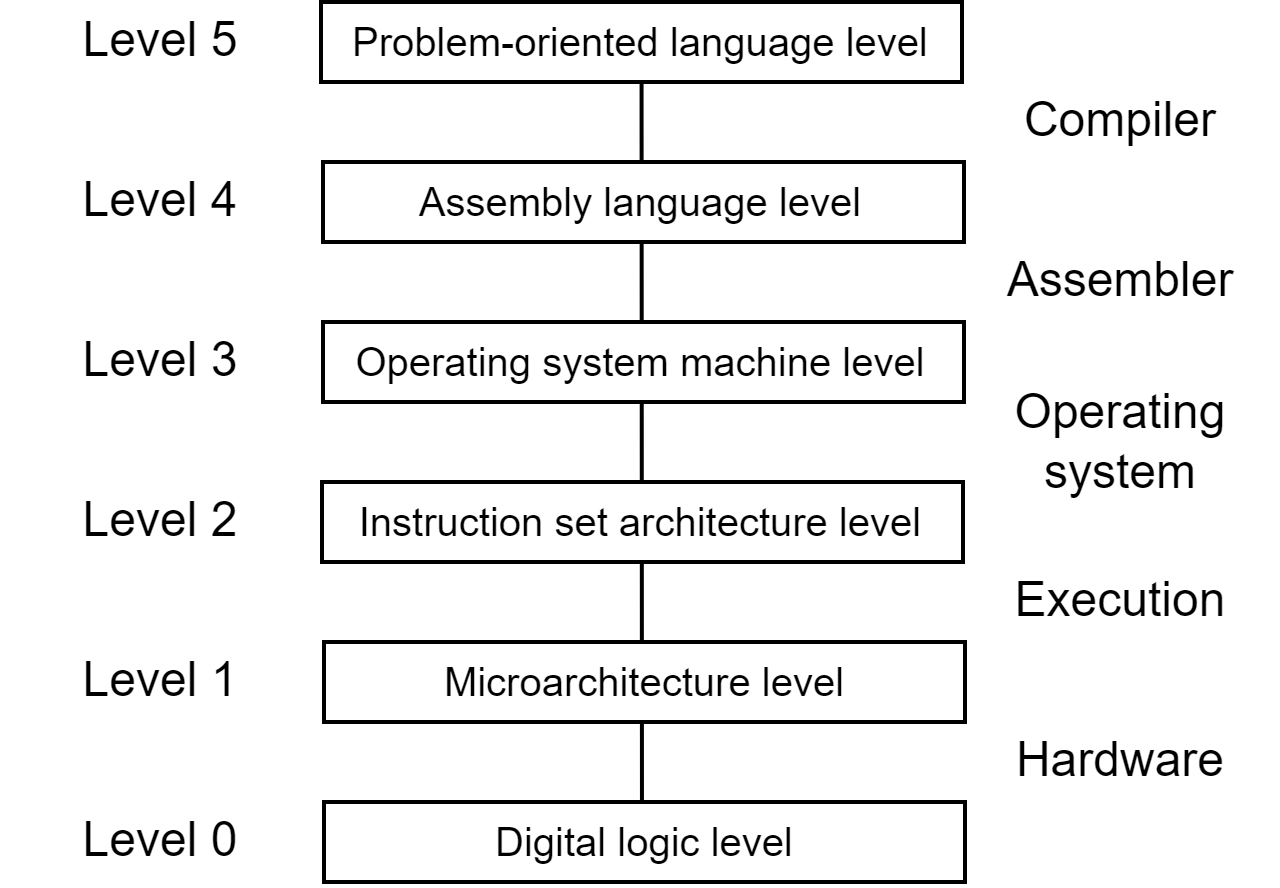
\includegraphics[width=0.5\linewidth]{images/lev.png}
    \caption{Machine levels}
\end{figure}

\paragraph*{Instruction set architecture}
The Instruction Set Architecture (ISA) corresponds to level two in the layered execution model and serves as the boundary between hardware and software.
There are two main aspects of ISA:
\begin{itemize}
    \item \textit{User ISA}: these are aspects of the ISA visible to an application program. 
        This includes operations such as addition, multiplication, logical operations, branching, etc. When an application interacts directly with the hardware, it uses the User ISA.
    \item \textit{System ISA}: these are aspects visible to supervisor software, such as the operating system (OS), which manages hardware resources. 
        The System ISA is responsible for hiding the complexity of CPUs, defining how applications access memory, and facilitating communication with the hardware. 
        When the OS interacts with the hardware (e.g., through drivers, memory management, scheduling), it uses the System ISA.
\end{itemize}

\paragraph*{Application binary interface}
The Application Binary Interface corresponds to level three in the layered execution model.
Under the User ISA, the ABI encompasses aspects of the ISA visible to an application program, such as arithmetic operations, logical operations, and branching.
System calls facilitate program interaction with shared hardware resources indirectly through the operating system. 
These calls enable applications to access hardware functionalities managed by the OS.
It's important to note that each machine level can only execute instructions intended for it, ensuring proper execution and interaction within the layered execution model.

\subsection{Machine virtualization}
A Virtual Machine serves as a logical abstraction, offering a virtualized execution environment. 
Specifically, a Virtual Machine:
\begin{itemize}
    \item Provides identical software behavior to that of a physical machine.
    \item Comprises a combination of physical hardware and virtualizing software.
    \item May present different resources than those of a physical machine.
    \item May result in varying levels of performance compared to physical counterparts.
\end{itemize}
The tasks of a Virtual Machine include:
\begin{itemize}
    \item Mapping virtual resources or states to corresponding physical ones.
    \item Utilizing physical machine instructions or calls to execute virtual instructions.
\end{itemize}
There are two primary types of Virtual Machines:
\begin{enumerate}
    \item \textit{System Virtual Machines}: these emulate an entire physical computer system, including its hardware resources.
    \item \textit{Process Virtual Machines}: these provide a virtualized environment for individual processes, allowing them to execute independently of the underlying hardware.
\end{enumerate}
The Virtual Machine Monitor supports levels zero-two of the architecture, facilitating the execution and management of virtualized environments.

\paragraph*{System virtual machines}
System virtual machines offer a complete system environment capable of supporting an operating system along with potentially numerous user processes. 
They grant the operating system running within them access to underlying hardware resources such as networking, I/O, and graphical user interface functionalities.
The virtualizing software, positioned between the hardware and software layers, emulates the Instruction Set Architecture interface perceived by software. 
This virtualization software is commonly referred to as the Virtual Machine Monitor.
The Virtual Machine Monitor can provide its functionality by operating directly on the hardware or by running on top of another operating system.

\paragraph*{Process virtual machines}
Process virtual machines are designed to support individual processes within an operating system environment. 
Here are some key characteristics:
\begin{itemize}
    \item The virtualizing software is positioned at the Application Binary Interface interface, sitting atop the combination of the operating system and hardware.
    \item This software emulates both user-level instructions and operating system calls, allowing processes to execute independently within the virtualized environment.
    \item Process virtualization software is commonly referred to as Runtime Software.
\end{itemize}
The runtime software supporting Process Virtual Machines typically encompasses levels zero-three of the architecture, facilitating the execution and management of individual processes within the virtualized environment.

\subsection{Virtualization taxonomy}
\begin{definition}[\textit{Host}]
    The host is the underlying platform that supports the virtualized environment/system.
\end{definition}
\begin{definition}[\textit{Guest}]
    The guest is the software that operates within the Virtual Machine environment as the guest.
\end{definition}
\begin{figure}[H]
    \centering
    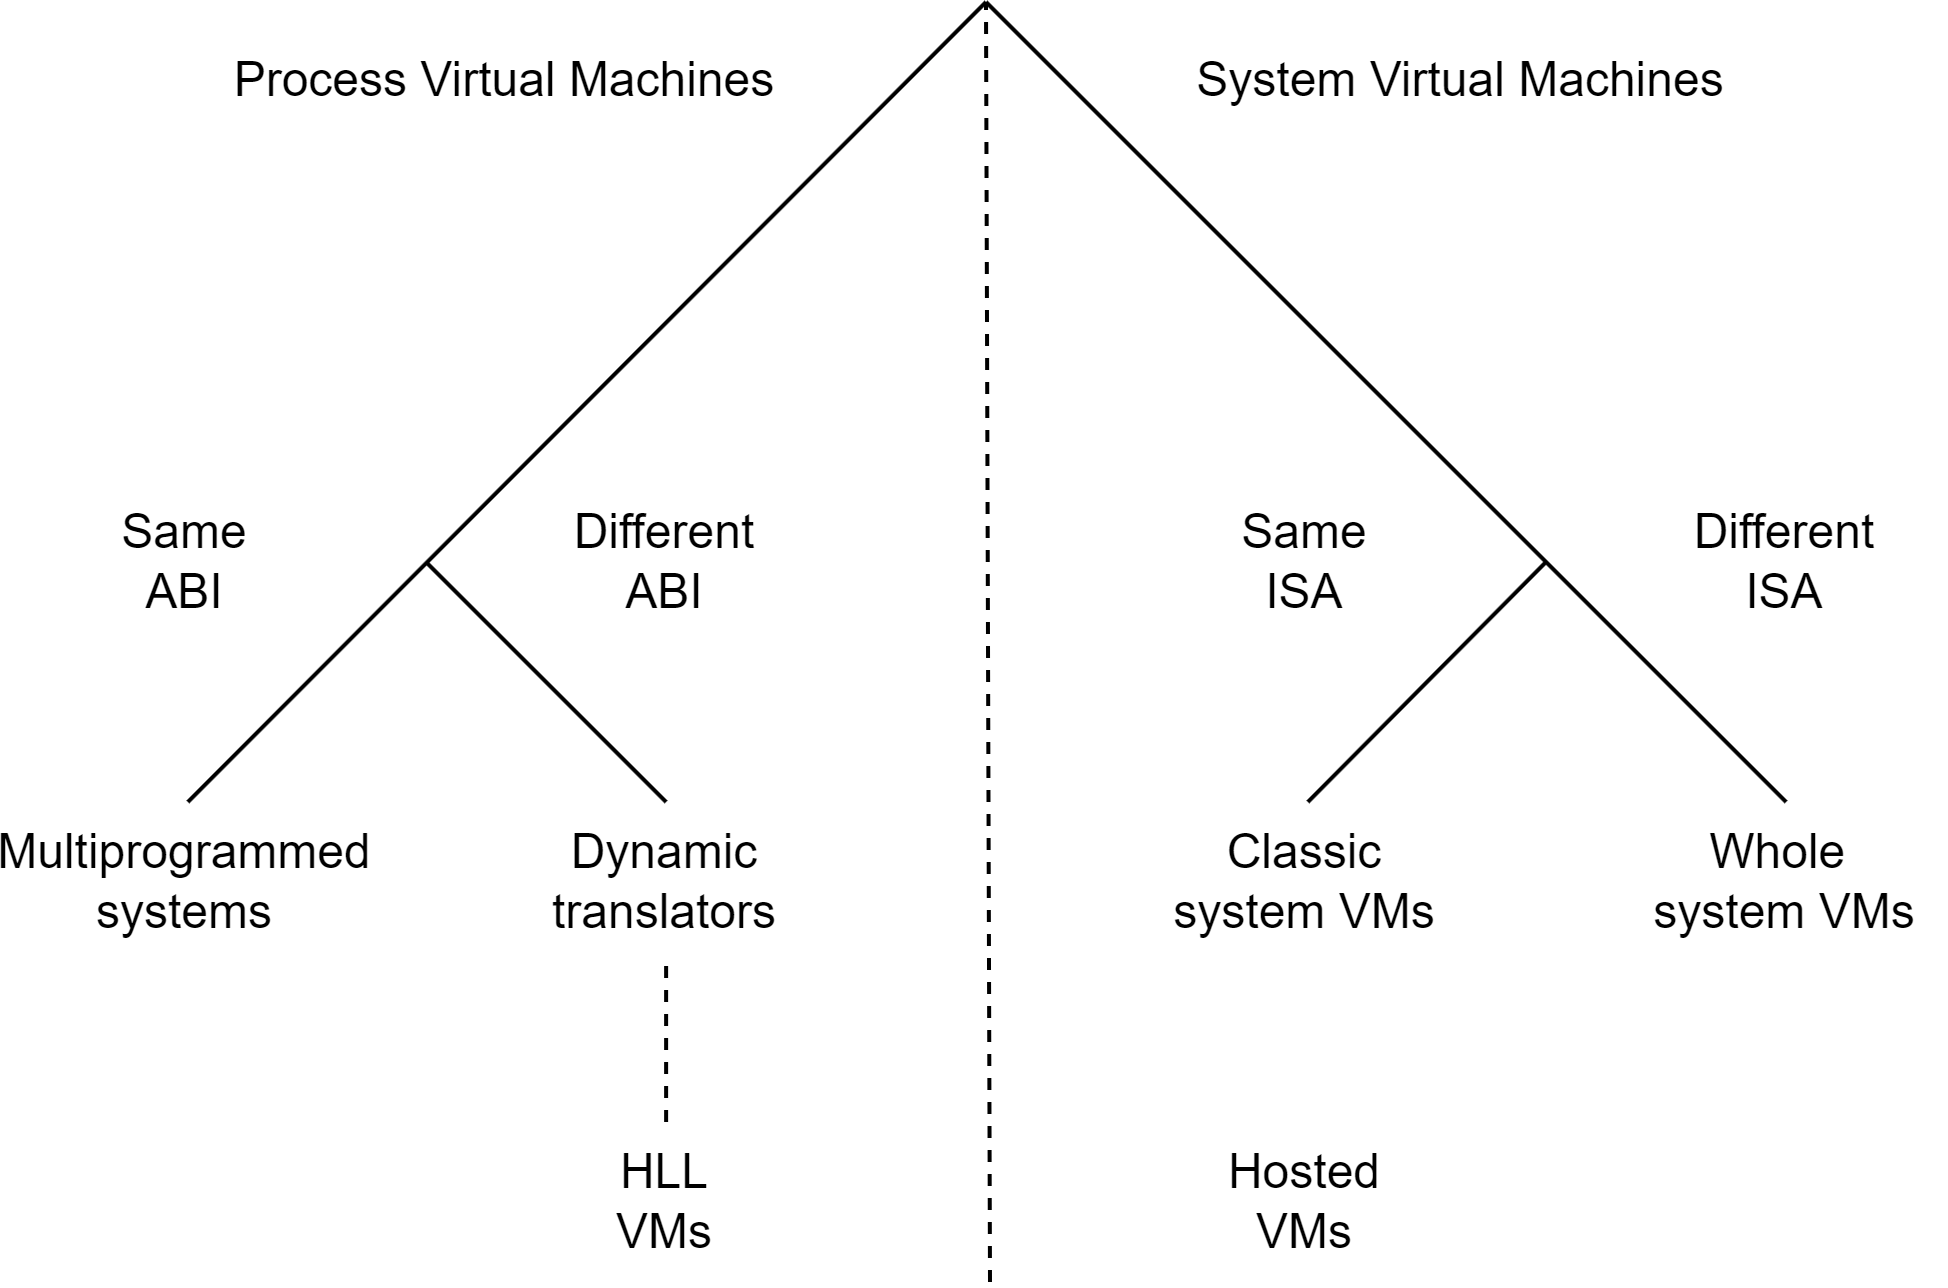
\includegraphics[width=0.5\linewidth]{images/vtyp.png}
    \caption{Types of virtualization}
\end{figure}

\paragraph*{Multiprogrammed systems}
In multiprogrammed systems with the same Application Binary Interface and operating system, Virtual Machines are formed by the combination of the OS call interface and the user Instruction Set Architecture. 
This approach is commonly adopted in modern operating systems to support multiple users.
The OS typically utilizes a Task/Process Manager for this purpose.
Each user process within this setup is provided with the illusion of having exclusive access to a complete machine. 
They are allocated their own address space and granted access to a file structure. 
The OS employs timesharing and manages hardware resources to facilitate this functionality. 
It can be argued that this configuration represents a form of virtualization.

\paragraph*{Emulation}
Emulation involves the development of software technologies designed to enable an application or operating system to operate in an environment different from its originally intended platform. 
This becomes necessary when Virtual Machines possess a different Instruction Set Architecture or Application Binary Interface compared to the architecture on which they are running.
An emulator thoroughly reads all the bytes contained within the memory of the system it seeks to replicate. 
One common approach to emulation is interpretation, wherein an interpreter program sequentially fetches, decodes, and emulates the execution of individual source instructions. 
However, this method can often be sluggish.

\paragraph*{High-Level Language VM}
The High-Level Language Virtual Machine (VM) aims to provide an isolated execution environment for each application or multiple instances of the same application. 
Its tasks involve translating application bytecode into OS-specific executable code while minimizing hardware and OS-specific features to ensure platform independence.
Applications running within this environment operate normally but exhibit certain characteristics:
\begin{itemize}
    \item They are sand-boxed, ensuring isolation from other processes.
    \item They have the capability to migrate between different environments.
    \item They do not conflict with one another.
    \item They do not adhere to traditional installation processes.
\end{itemize}
An illustrative example of a High-Level Language VM is the Java Virtual Machine, which enables Java applications to function on any architecture supported by an interpreter, such as the Java Runtime Environment.

\paragraph*{Classic system virtual machine}
In the context of classic system virtual machines operating with the same Instruction Set Architecture (ISA):
\begin{itemize}
    \item The Virtual Machine Monitor (VMM) resides directly on bare hardware, serving as the foundation for the virtual machines.
    \item The VMM possesses the capability to intercept interactions between guest operating systems (OSs) and hardware resources.
    \item This architecture represents one of the most efficient VM configurations, as hardware execution aligns with that of the virtual machines (VMs).
\end{itemize}
It facilitates the execution of two different OSs on the same hardware platform.

\paragraph*{System virtual machines}
System virtual machines can be classified into two categories:
\begin{itemize}
    \item \textit{Hosted VMs}: in this setup, the virtualizing software operates on top of an existing host operating system.
    \item \textit{Whole-system VMs}: these virtualize all software components. As the Instruction Set Architectures (ISAs) may differ, both application and OS code require emulation, typically achieved through binary translation. 
        Native execution is not possible in this scenario.
\end{itemize}
The Virtual Machine Monitor (VMM) and guest software are typically implemented on top of a conventional host OS running on the hardware.
The VM software must emulate the entire hardware environment and all guest ISA operations to equivalent OS calls to the host.
An example scenario would be Microsoft Word and Windows running on a PowerPC architecture (not x86 family).

\subsection{Implementation}
In the context of implementing virtualization within a typical layered architecture of a system, additional layers are introduced between execution stack layers. 
Depending on the placement of these new layers, various types of virtualization can be achieved.

\paragraph*{Hardware-level virtualization:}
Hardware-level virtualization involves placing the virtualization layer between the hardware and the operating system. 
This positioning alters the interface seen by the OS and applications, potentially differing from the physical hardware interface.

\paragraph*{Application-level virtualization}
In application-level virtualization, a virtualization layer is inserted between the operating system and specific applications.
This layer ensures that applications are provided with a consistent interface, regardless of the underlying OS. 
As a result, applications can run within their own environment, independent of the OS.

\paragraph*{System-level virtualization}
In system-level virtualization, the virtualization layer offers the interface of a physical machine to a secondary operating system and a set of applications running within it. 
This enables them to operate atop an existing OS. 
This virtualization layer is positioned between the system's primary OS and other OS instances.
These platforms facilitate the execution of multiple operating systems on a single hardware infrastructure.

\paragraph*{Properties}
Virtual Machines possess several significant properties:
\begin{itemize}
    \item \textit{Partitioning}: multiple operating systems can execute on a single physical machine, with resources partitioned among the different VMs.
    \item \textit{Isolation}: VMs provide fault tolerance and security at the hardware level by ensuring isolation between them.
    \item \textit{Advanced resource control}: hypervisors manage resources to guarantee performance.
    \item \textit{Encapsulation}: the entire state of a VM can be saved in a file, allowing VMs to be copied and moved easily, simplifying replication and migration processes.
    \item \textit{Hardware independence}: all VMs perceive the same virtual hardware, regardless of the underlying host system. 
        This simplifies provisioning and migration of VMs.
\end{itemize}
These properties have been instrumental in the emergence of cloud computing and the development of many services used today.

\subsection{Virtual machine managers}
Virtual Machine Manager (VMM), also known as Virtual Machine Monitor (VMM) or Hypervisor, is an application responsible for:
\begin{itemize}
    \item Managing virtual machines.
    \item Mediating access to hardware resources on the physical host system.
    \item Intercepting and handling any privileged or protected instructions issued by the virtual machines.
    \item Typically running virtual machines with operating systems, libraries, and utilities compiled for the same type of processor and instruction set as the physical machine.
\end{itemize}
These managers are crucial for supporting Cloud Computing. 
While the terms VMM, Hypervisor, and Virtual Machine Manager are often used interchangeably, some authors attribute slightly different meanings to each:
\begin{itemize}
    \item \textit{Virtual machine monitor}: refers to the virtualization software.
    \item \textit{Hypervisor}: denotes a virtualization software that runs directly on the hardware.
    \item \textit{Virtual machine manager}: a VMM or Hypervisor used to create, configure, and maintain virtualized resources. 
        It provides a user-friendly interface to the underlying virtualization software.
\end{itemize}
\begin{figure}[H]
    \centering
    \begin{subfigure}{0.49\textwidth}
        \centering
        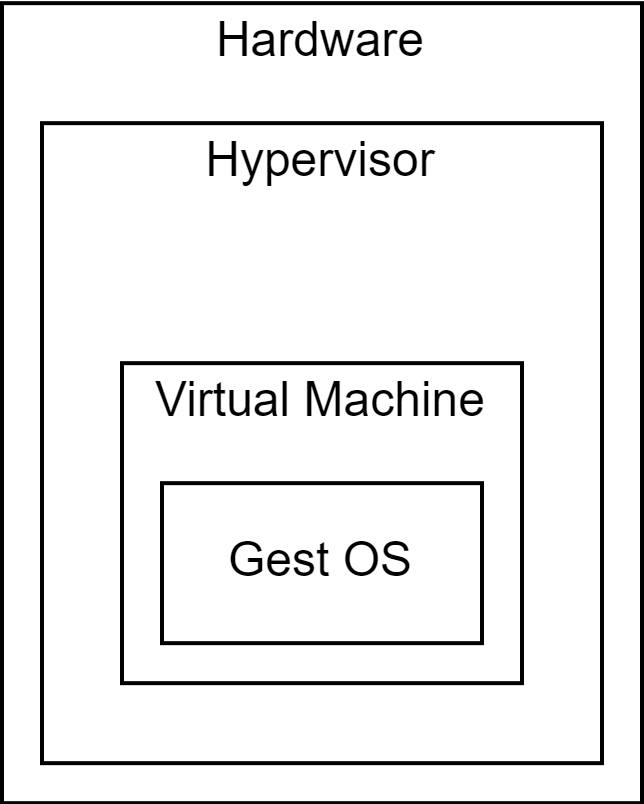
\includegraphics[width=0.75\linewidth]{images/hyp1.png} 
        \caption{Hypervisor type 1}
    \end{subfigure}
    \begin{subfigure}{0.49\textwidth}
        \centering
        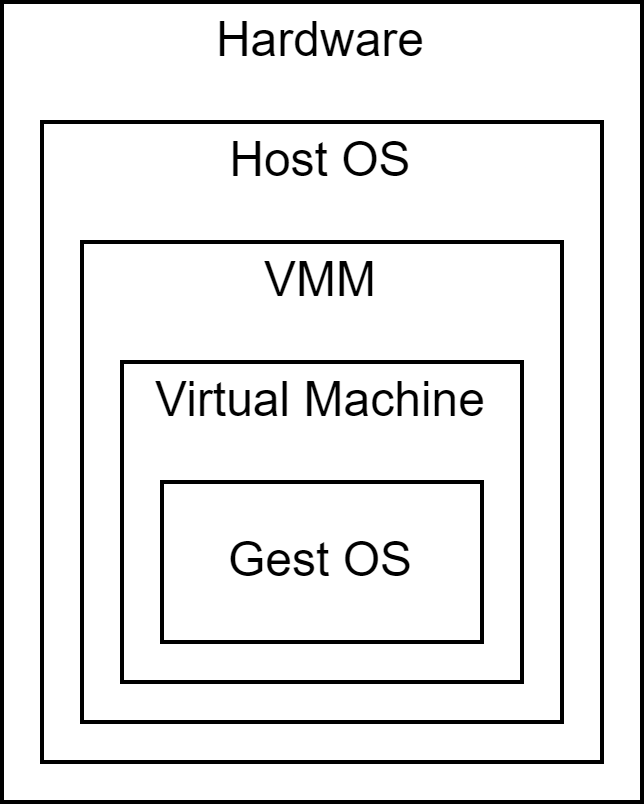
\includegraphics[width=0.75\linewidth]{images/hyp2.png}
        \caption{Hypervisor type 2}
    \end{subfigure}
    \caption{Type one hypervisor architectures}
\end{figure}

\paragraph*{Type 1 hypervisor}
Type 1 hypervisors, also known as bare-metal hypervisors, directly control the hardware without requiring an underlying operating system. 
The architecture of Type 1 hypervisors can be categorized into two main types:
\begin{enumerate}
    \item \textit{Monolithic}: in this architecture, device drivers run within the hypervisor itself. 
        This approach offers better performance and isolation but is limited to hardware for which the hypervisor has drivers.
    \item \textit{Microkernel}: here, device drivers run within a service virtual machine. 
        This results in a smaller hypervisor and leverages the driver ecosystem of an existing operating system. 
        It also allows the use of third-party drivers, although recompilation may be necessary.
\end{enumerate}
\begin{figure}[H]
    \centering
    \begin{subfigure}{0.49\textwidth}
        \centering
        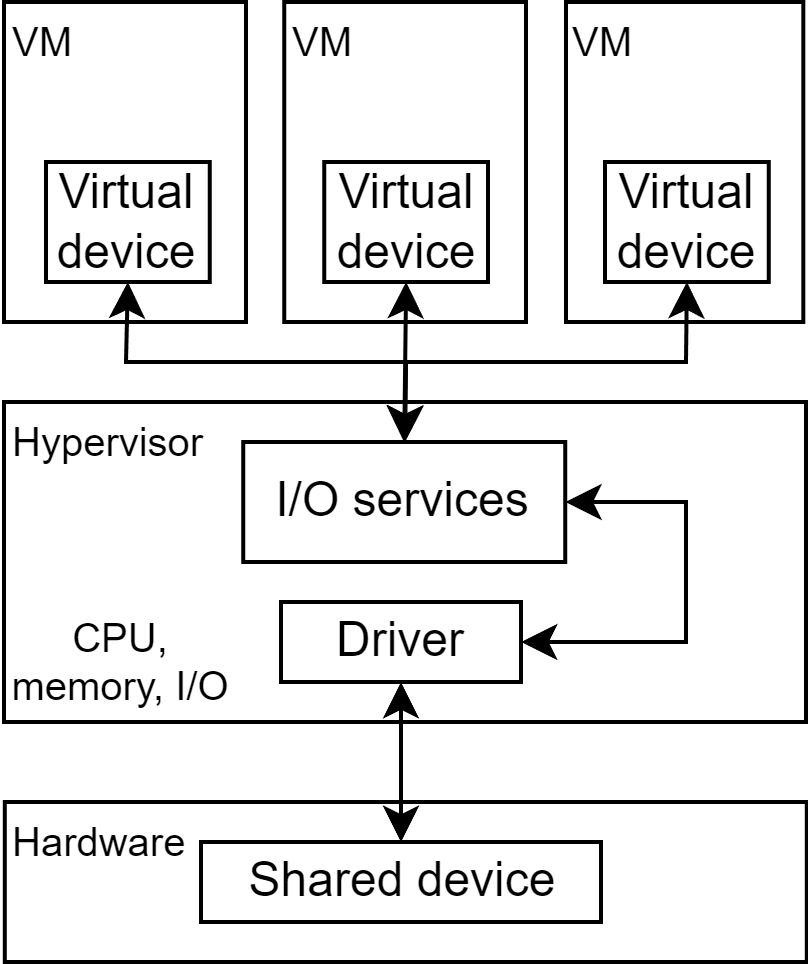
\includegraphics[width=0.75\linewidth]{images/mono.png} 
        \caption{Monolithic architecture}
    \end{subfigure}
    \begin{subfigure}{0.49\textwidth}
        \centering
        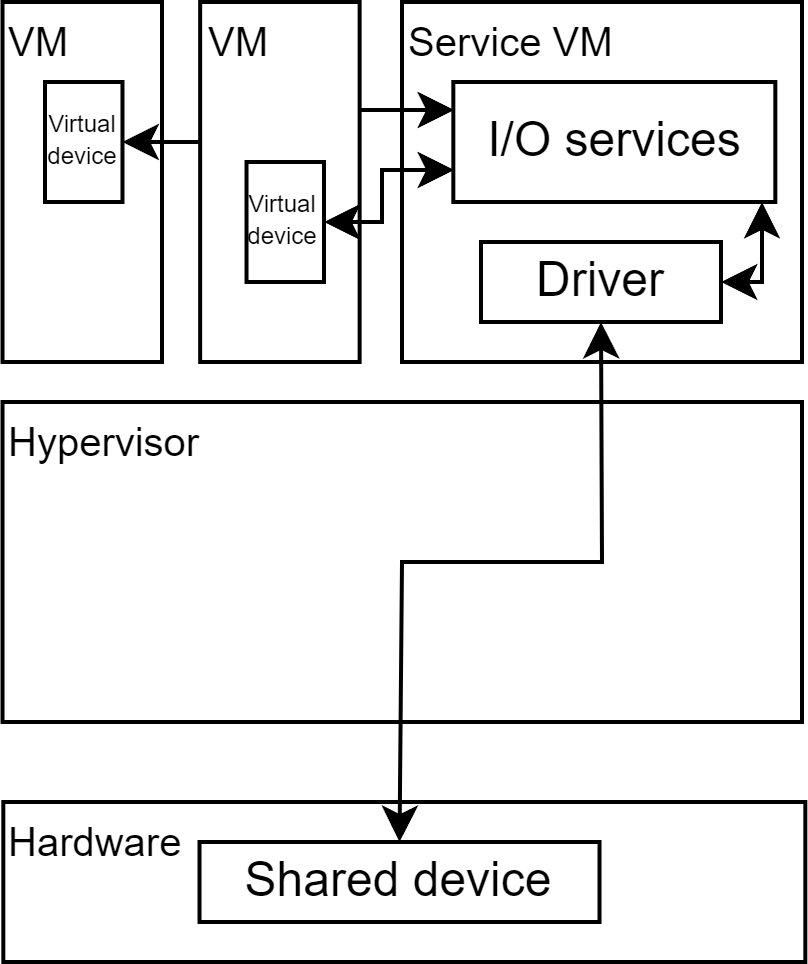
\includegraphics[width=0.75\linewidth]{images/mic.png}
        \caption{Microkernel architecture}
    \end{subfigure}
    \caption{Type one hypervisor architectures}
\end{figure}

Type 1 hypervisors are sometimes utilized to provide workarounds for certain operating systems. 
Two notable examples include: enabling Windows to function legitimately without an official license, or facilitating the installation of Mac OS on non-Apple hardware. 

\paragraph*{Type two hypervisor}
Type 2 hypervisors, also known as hosted hypervisors or VMMs (Virtual Machine Monitors), are situated within a host operating system. 
They utilize the code of the host OS for functions like CPU scheduling and memory management.
In systems employing Type 2 hypervisors, there are typically two operating systems operating on the same hardware: the Host OS, which manages the hardware of the system, and the Guest OS, which runs within the virtual machine.
The Type 2 hypervisor operates within the Host OS, while applications execute within the Guest OS.
Key characteristics of Type 2 hypervisors include:
\begin{itemize}
    \item Dependency on a Host OS to manage the hardware on which the VMM operates.
    \item Flexibility in terms of underlying hardware.
    \item Ease of management and configuration, with the VMM being able to utilize the Host OS to provide a graphical user interface beyond BIOS.
    \item Need for caution to prevent conflicts between the Host OS and Guest OS, especially in areas like virtual memory management.
    \item Consumption of a portion of physical resources by the Host OS, such as a dedicated core.
\end{itemize}

\subsection{Virtualization techniques}
There are various methods to implement system-level virtualization with the same Instruction Set Architecture. 
Two prominent techniques are paravirtualization and full virtualization.

\paragraph*{Paravirtualization}
Paravirtualization entails a collaborative effort between the guest operating system and the Virtual Machine Monitor. 
Unlike full virtualization, the VMM provides a virtual interface to virtual machines that closely resembles but is not identical to the underlying hardware. 
This approach aims to diminish the guest's execution of tasks that are resource-intensive in the virtualized environment by enabling the guest and host to communicate through designated"hooks.
Advantages of Paravirtualization include a simpler VMM implementation and enhanced performance due to reduced overhead. 
However, it necessitates modifications to the guest OS and is incompatible with traditional operating systems, being available only on certain Linux releases.

\paragraph*{Full Virtualization}
Full Virtualization provides a complete simulation of the underlying hardware, encompassing the entire instruction set, input/output operations, interrupts, and memory access. 
Protected instructions are intercepted and managed by the Hypervisor.
Advantages include the capability to run unmodified operating systems. 
However, drawbacks entail dependence on Hypervisor mediation to facilitate communication between guests and hosts for tasks that would otherwise occur in the virtual domain, and limited compatibility across architectures, necessitating specific hardware support.
\begin{figure}[H]
    \centering
    \begin{subfigure}{0.49\textwidth}
        \centering
        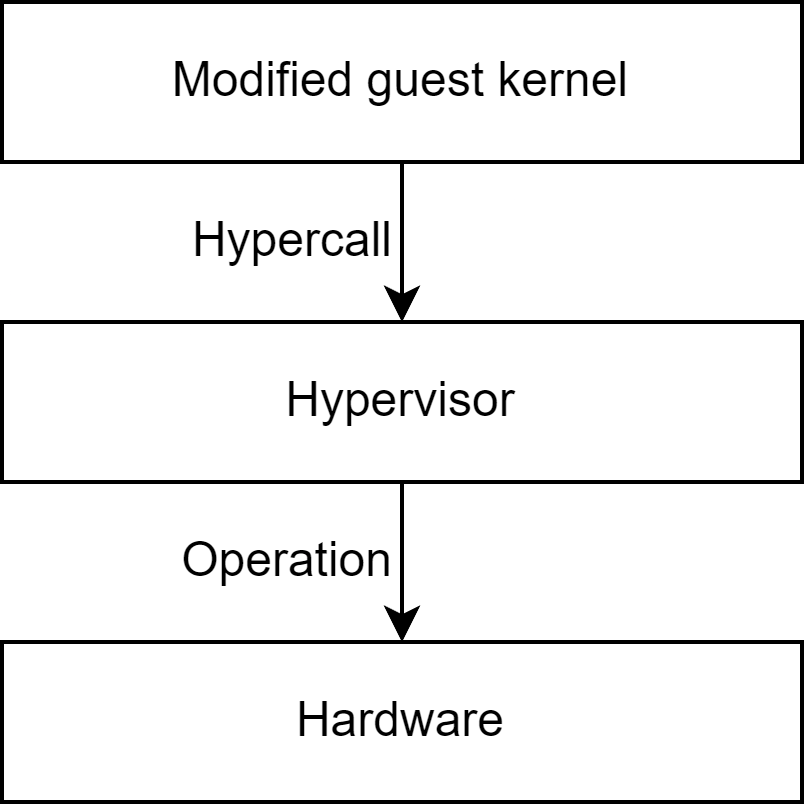
\includegraphics[width=0.75\linewidth]{images/para.png} 
        \caption{Paravirtualization}
    \end{subfigure}
    \begin{subfigure}{0.49\textwidth}
        \centering
        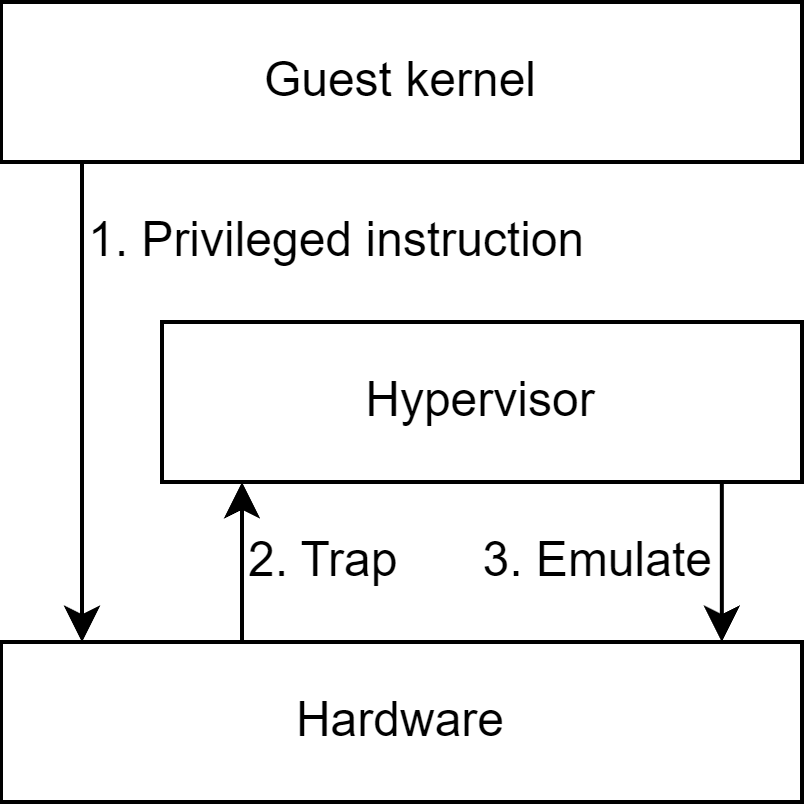
\includegraphics[width=0.75\linewidth]{images/full.png}
        \caption{Full virtualization}
    \end{subfigure}
    \caption{Comparison of paravirtualization and full virtualization}
\end{figure}

\subsection{Containers}
Containers serve as lightweight virtualization solutions, particularly significant in DevOps contexts. 
They encapsulate pre-configured packages containing all necessary components for code execution, including code, libraries, variables, and configurations, within the target machine.

Their primary advantage lies in predictable, repeatable, and immutable behavior. 
When duplicating a master container onto another server, its execution remains consistent and error-free across environments.

For instance, consider a website container. 
Rather than exporting/importing development/test/production environments separately, a container containing the site can be created and deployed to the destination environment.

Contrasting containers with virtual machines, the former offer virtualization at the operating system level, sharing the host system kernel with other containers. 
In contrast, virtual machines provide hardware virtualization, with applications dependent on guest operating systems.

\paragraph*{Characteristics}
Containers possess several key characteristics:
\begin{itemize}
    \item \textit{Flexibility}: they can containerize even complex applications.
    \item \textit{Lightweight}: containers leverage and share the host kernel, minimizing resource usage.
    \item \textit{Interchangeable}: updates can be seamlessly distributed without disruption.
    \item \textit{Portable}: they can be created locally, deployed in the cloud, and run anywhere.
    \item \textit{Scalable}: containers enable automatic replication and distribution of replicas.
    \item \textit{Stackable}: they can be vertically stacked and deployed on the fly.
\end{itemize}
Containers streamline application deployment, enhance scalability, and promote modular application development, where modules remain independent and uncoupled.
Containers find various applications, including:
\begin{itemize}
    \item Accelerating local development and build workflows, making them faster, more efficient, and lightweight.
    \item Consistently running stand-alone services and applications across multiple environments.
    \item Creating isolated instances for running tests.
    \item Building and testing complex applications and architectures locally before deployment to production environments.
    \item Establishing multi-user Platform-as-a-Service (PaaS) infrastructures.
    \item Providing lightweight sandbox environments for developing, testing, and teaching technologies, such as the Unix shell or a programming language.
    \item Implementing Software as a Service (SaaS) applications.
    \item Developing Function as a Service (FaaS) applications.
\end{itemize}

\paragraph*{Docker}
Docker simplifies software deployment by utilizing containers:
Docker is an open-source platform that facilitates the building, shipping, and running of applications across diverse environments.
It operates based on DockerFiles, which are textual files containing commands to assemble application images via the command line.
These DockerFiles define a compilation process. 
When executed with the Docker build command, they create immutable Docker images—snapshots of the application.
Containers created with Docker can be run on various platforms, such as laptops, servers, cloud environments, or Raspberry Pi devices.
Regardless of the hosting environment, Docker ensures consistent behavior for containers.
Docker Swarm, an orchestration tool integrated into the Docker ecosystem, aids in container management and scaling.

\paragraph*{Kubernetes}
Kubernetes, an open-source project from Google, is well-suited for managing medium to large clusters and complex applications.
It offers a comprehensive and customizable solution for efficiently coordinating large-scale node clusters in production:
Kubernetes enables running containers across diverse machines within a cluster.
It allows for scaling the performance of applications by adjusting the number of containers dynamically.
Load balancing capabilities distribute workloads effectively among containers.
In the event of machine failure, Kubernetes can automatically initiate new containers on alternative machines, ensuring continuous operation.